\documentclass[11pt,a4paper]{report}
\usepackage[textwidth=37em,vmargin=30mm]{geometry}
\usepackage{calc,xunicode,amsmath,amssymb,paralist,enumitem,tabu,booktabs,datetime2,xeCJK,xeCJKfntef,listings}
\usepackage{tocloft,fancyhdr,tcolorbox,xcolor,graphicx,eso-pic,xltxtra,xelatexemoji}

\newcommand{\envyear}[0]{2024}
\newcommand{\envdatestr}[0]{2024-10-26}
\newcommand{\envfinaldir}[0]{webdb/2024/20241026/final}

\usepackage[hidelinks]{hyperref}
\hypersetup{
    colorlinks=false,
    pdfpagemode=FullScreen,
    pdftitle={Web Digest - \envdatestr}
}

\setlength{\cftbeforechapskip}{10pt}
\renewcommand{\cftchapfont}{\rmfamily\bfseries\large\raggedright}
\setlength{\cftbeforesecskip}{2pt}
\renewcommand{\cftsecfont}{\sffamily\small\raggedright}

\setdefaultleftmargin{2em}{2em}{1em}{1em}{1em}{1em}

\usepackage{xeCJK,xeCJKfntef}
\xeCJKsetup{PunctStyle=plain,RubberPunctSkip=false,CJKglue=\strut\hskip 0pt plus 0.1em minus 0.05em,CJKecglue=\strut\hskip 0.22em plus 0.2em}
\XeTeXlinebreaklocale "zh"
\XeTeXlinebreakskip = 0pt


\setmainfont{Brygada 1918}
\setromanfont{Brygada 1918}
\setsansfont{IBM Plex Sans}
\setmonofont{JetBrains Mono NL}
\setCJKmainfont{Noto Serif CJK SC}
\setCJKromanfont{Noto Serif CJK SC}
\setCJKsansfont{Noto Sans CJK SC}
\setCJKmonofont{Noto Sans CJK SC}

\setlength{\parindent}{0pt}
\setlength{\parskip}{8pt}
\linespread{1.15}

\lstset{
	basicstyle=\ttfamily\footnotesize,
	numbersep=5pt,
	backgroundcolor=\color{black!5},
	showspaces=false,
	showstringspaces=false,
	showtabs=false,
	tabsize=2,
	captionpos=b,
	breaklines=true,
	breakatwhitespace=true,
	breakautoindent=true,
	linewidth=\textwidth
}






\newcommand{\coverpic}[2]{
    % argv: itemurl, authorname
    Cover photo by #2~~(\href{#1}{#1})
}
\newcommand{\makeheader}[0]{
    \begin{titlepage}
        % \newgeometry{hmargin=15mm,tmargin=21mm,bmargin=12mm}
        \begin{center}
            
            \rmfamily\scshape
            \fontspec{BaskervilleF}
            \fontspec{Old Standard}
            \fontsize{59pt}{70pt}\selectfont
            WEB\hfill DIGEST
            
            \vfill
            % \vskip 30pt
            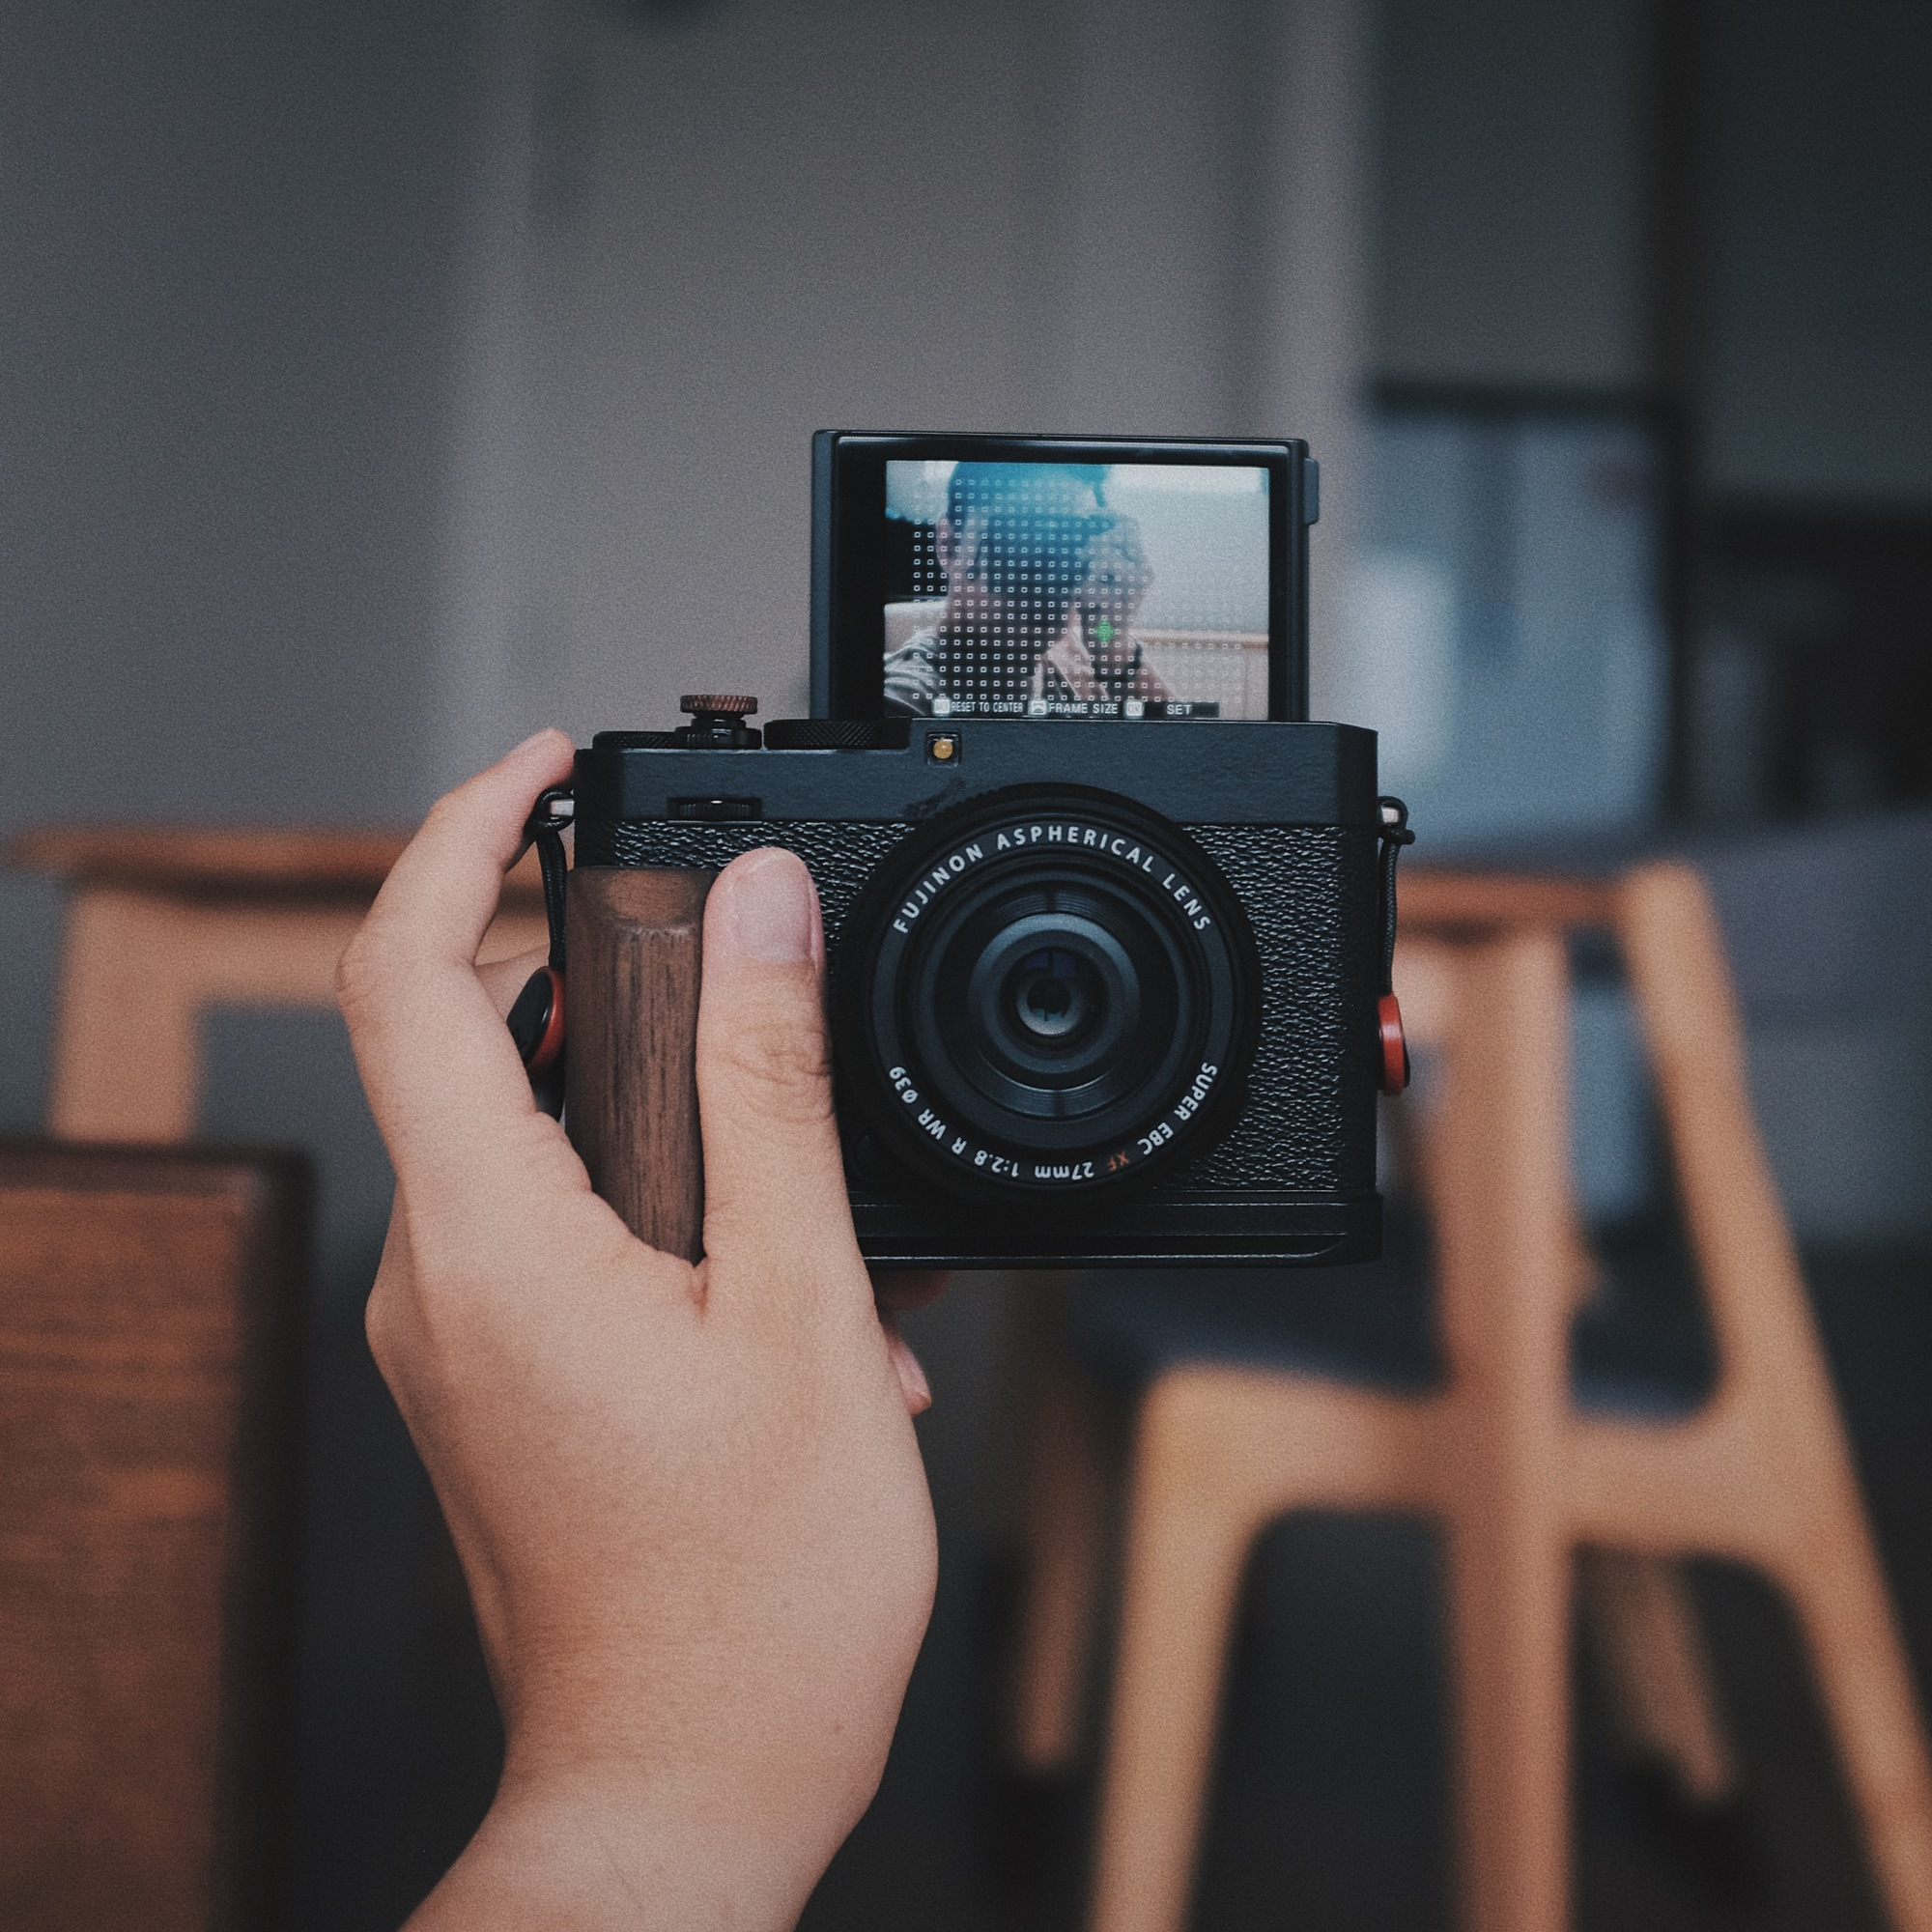
\includegraphics[width=\linewidth]{\envfinaldir/coverpic-prod.jpg}\par
            % \vskip 30pt
            \vfill

            \normalsize\rmfamily\scshape
            \copyright{} The Web Digest Project \hfill\large \envdatestr
        \end{center}
    \end{titlepage}
    % \restoregeometry
}
\newcommand{\simplehref}[1]{%
    \textcolor{blue!80!green}{\href{#1}{#1}}%
}
\renewcommand{\contentsname}{\center\Huge\sffamily\bfseries Contents\par\vskip 20pt}
\newcounter{ipartcounter}
\setcounter{ipartcounter}{0}
\newcommand{\ipart}[1]{
    % \vskip 20pt
    \clearpage
    \stepcounter{ipartcounter}
    \phantomsection
    \addcontentsline{toc}{chapter}{#1}
    % \begin{center}
    %     \Huge
    %     \sffamily\bfseries
    %     #1
    % \end{center}
    % \vskip 20pt plus 7pt
}
\newcounter{ichaptercounter}
\setcounter{ichaptercounter}{0}
\newcommand{\ichapter}[1]{
    % \vskip 20pt
    \clearpage
    \stepcounter{ichaptercounter}
    \phantomsection
    \addcontentsline{toc}{section}{\numberline{\arabic{ichaptercounter}}#1}
    \begin{center}
        \Huge
        \sffamily\bfseries
        #1
    \end{center}
    \vskip 20pt plus 7pt
}
\newcommand{\entrytitlefont}[1]{\subsection*{\raggedright\Large\sffamily\bfseries#1}}
\newcommand{\entryitemGeneric}[2]{
    % argv: title, url
    \parbox{\linewidth}{
        \entrytitlefont{#1}\par\vskip 5pt
        \footnotesize\ttfamily\mdseries
        \simplehref{#2}
    }\vskip 11pt plus 11pt minus 1pt
}
\newcommand{\entryitemGithub}[3]{
    % argv: title, url, desc
    \parbox{\linewidth}{
        \entrytitlefont{#1}\par\vskip 5pt
        \footnotesize\ttfamily\mdseries
        \simplehref{#2}\par\vskip 5pt
        \small\rmfamily\mdseries#3
    }\vskip 11pt plus 11pt minus 1pt
}
\newcommand{\entryitemAp}[3]{
    % argv: title, url, desc
    \parbox{\linewidth}{
        \entrytitlefont{#1}\par\vskip 5pt
        \footnotesize\ttfamily\mdseries
        \simplehref{#2}\par\vskip 5pt
        \small\rmfamily\mdseries#3
    }\vskip 11pt plus 11pt minus 1pt
}
\newcommand{\entryitemHackernews}[3]{
    % argv: title, hnurl, rawurl
    % \parbox{\linewidth}{
    %     \entrytitlefont{#1}\par\vskip 5pt
    %     \footnotesize\ttfamily\mdseries
    %     \simplehref{#3}\par
    %     \textcolor{black!50}{\href{#2}{#2}}
    % }\vskip 11pt plus 11pt minus 1pt
    \begin{minipage}{\linewidth}
            \entrytitlefont{#1}\par\vskip 5pt
            \footnotesize\ttfamily\mdseries
            \simplehref{#3}\par
            \textcolor{black!50}{\href{#2}{#2}}
    \end{minipage}\par\vskip 11pt plus 11pt minus 1pt
}







\begin{document}

\makeheader

\tableofcontents\clearpage




\ipart{Developers}
\ichapter{Hacker News}
\entryitemTwoLinks{Jeff Bezos killed Washington Post endorsement of Kamala Harris}{https://news.ycombinator.com/item?id=41949297}{https://www.cnbc.com/2024/10/25/jeff-bezos-killed-washington-post-endorsement-of-kamala-harris-.html}

\entryitemTwoLinks{We can now fix McDonald's ice cream machines}{https://news.ycombinator.com/item?id=41949098}{https://www.ifixit.com/News/102368/victory-is-sweet-we-can-now-fix-mcdonalds-ice-cream-machines}

\entryitemTwoLinks{Company named "><SCRIPT SRC=HTTPS://MJT.XSS.HT> LTD" forced to change it (2020)}{https://news.ycombinator.com/item?id=41948666}{https://www.theguardian.com/uk-news/2020/nov/06/companies-house-forces-business-name-change-to-prevent-security-risk}

\entryitemTwoLinks{Detecting when LLMs are uncertain}{https://news.ycombinator.com/item?id=41947566}{https://www.thariq.io/blog/entropix/}

\entryitemTwoLinks{Infinite Git repos on Cloudflare workers}{https://news.ycombinator.com/item?id=41947513}{https://gitlip.com/blog/infinite-git-repos-on-cloudflare-workers}

\entryitemTwoLinks{Universal optimality of Dijkstra via beyond-worst-case heaps}{https://news.ycombinator.com/item?id=41947355}{https://arxiv.org/abs/2311.11793}

\entryitemTwoLinks{Disposable vapes to be banned in England and Wales}{https://news.ycombinator.com/item?id=41946401}{https://www.bbc.com/news/articles/cd7n3zyp114o}

\entryitemTwoLinks{Smartphone buyers meh on AI, care more about battery life}{https://news.ycombinator.com/item?id=41946188}{https://www.cnet.com/tech/mobile/with-apple-intelligence-on-the-horizon-a-quarter-of-smartphone-owners-are-unimpressed-by-ai/}

\entryitemTwoLinks{Battleships Logic Puzzle}{https://news.ycombinator.com/item?id=41946036}{https://lukerissacher.com/battleships}

\entryitemTwoLinks{A deep dive into Linux's new mseal syscall}{https://news.ycombinator.com/item?id=41945894}{https://blog.trailofbits.com/2024/10/25/a-deep-dive-into-linuxs-new-mseal-syscall/}

\entryitemTwoLinks{Plastic chemical phthalate causes DNA breakage, chromosome defects, study finds}{https://news.ycombinator.com/item?id=41945372}{https://medicalxpress.com/news/2024-10-plastic-chemical-phthalate-dna-breakage.html}

\entryitemTwoLinks{Category Theory Illustrated: Logic (2021)}{https://news.ycombinator.com/item?id=41945308}{https://abuseofnotation.github.io/category-theory-illustrated/05\_logic/}

\entryitemTwoLinks{Notes on the new Claude analysis JavaScript code execution tool}{https://news.ycombinator.com/item?id=41943662}{https://simonwillison.net/2024/Oct/24/claude-analysis-tool/}

\entryitemTwoLinks{Smarter Than 'Ctrl+F': Linking Directly to Web Page Content}{https://news.ycombinator.com/item?id=41943098}{https://alfy.blog/2024/10/19/linking-directly-to-web-page-content.html}

\entryitemTwoLinks{The brain's waste clearing lymphatic system shown in people for first time}{https://news.ycombinator.com/item?id=41942096}{https://www.nih.gov/news-events/nih-research-matters/brain-waste-clearance-system-shown-people-first-time}

\entryitemTwoLinks{Cerebras Inference now 3x faster: Llama3.1-70B breaks 2,100 tokens/s}{https://news.ycombinator.com/item?id=41941883}{https://cerebras.ai/blog/cerebras-inference-3x-faster}

\entryitemTwoLinks{OpenFeature – a vendor-agnostic, community-driven API for feature flagging}{https://news.ycombinator.com/item?id=41941493}{https://github.com/open-feature}

\entryitemTwoLinks{U.S. Consumer Watchdog Cautions Businesses on Surveillance of Workers}{https://news.ycombinator.com/item?id=41941052}{https://www.wsj.com/articles/u-s-consumer-watchdog-cautions-businesses-on-surveillance-of-workers-8262bee3}

\entryitemTwoLinks{Bitwarden SDK relicensed from proprietary to GPLv3}{https://news.ycombinator.com/item?id=41940580}{https://github.com/bitwarden/sdk-internal/commit/db648d7ea85878e9cce03283694d01d878481f6b}

\entryitemTwoLinks{ST Book, the Notebook Atari ST}{https://news.ycombinator.com/item?id=41940266}{https://www.goto10retro.com/p/st-book-the-notebook-atari-st}\ichapter{Phoronix}
\entryitemGeneric{\hskip 0pt{}Linux Fixes "Meltdown Lite" Mitigation Handling On Newer Zen 5 CPUs}{https://www.phoronix.com/news/Meltdown-Lite-Zen-5-Linux-Fix}

\entryitemGeneric{\hskip 0pt{}Intel Core Ultra 5 245K Linux Performance}{https://www.phoronix.com/review/intel-core-ultra-5-245k-linux}

\entryitemGeneric{\hskip 0pt{}AMDGPU Changes Readied For Linux 6.13: Runtime Repartitioning, Many Fixes}{https://www.phoronix.com/news/Linux-6.13-AMDGPU-Repart}

\entryitemGeneric{\hskip 0pt{}Linux Support Continues For The Now-Canceled Snapdragon X Elite Dev Kit For Windows}{https://www.phoronix.com/news/Snapdragon-X-Elite-Dev-Kit-Goes}

\entryitemGeneric{\hskip 0pt{}DRM Client Library Code Ready Ahead Of Linux 6.13}{https://www.phoronix.com/news/DRM-Client-Library-Linux-6.13}

\entryitemGeneric{\hskip 0pt{}FUTEX2 NUMA \& Small Futexes Revived For Linux}{https://www.phoronix.com/news/FUTEX2-NUMA-Small-Futex}

\entryitemGeneric{\hskip 0pt{}Cloud Hypervisor 42 Released With SVE/SVE2 Support For AArch64 Guests}{https://www.phoronix.com/news/Cloud-Hypervisor-42}

\entryitemGeneric{\hskip 0pt{}Intel Preps OA Sync, Panther Lake Workaround \& Other New Graphics Code For Linux 6.13}{https://www.phoronix.com/news/Intel-More-Xe-DRM-Linux-6.13}

\entryitemGeneric{\hskip 0pt{}Some Clarity On The Linux Kernel's "Compliance Requirements" Around Russian Sanctions}{https://www.phoronix.com/news/Linux-Compliance-Requirements}


\ipart{Developers~~~~(zh-Hans)}
\ichapter{Solidot}
\entryitemGeneric{\hskip 0pt{}超新星可能清理过太阳系}{https://www.solidot.org/story?sid=79595}

\entryitemGeneric{\hskip 0pt{}人口峰值可能会更快到来}{https://www.solidot.org/story?sid=79594}

\entryitemGeneric{\hskip 0pt{}蒂姆波顿称互联网让他倍感抑郁}{https://www.solidot.org/story?sid=79593}

\entryitemGeneric{\hskip 0pt{}Kroger 和沃尔玛否认会使用数字价格标签动态定价}{https://www.solidot.org/story?sid=79592}

\entryitemGeneric{\hskip 0pt{}Linux 项目根据 OFAC 制裁名单移除俄罗斯维护者}{https://www.solidot.org/story?sid=79591}

\entryitemGeneric{\hskip 0pt{}报告称中国 5 个行业产能超过全球需求}{https://www.solidot.org/story?sid=79590}

\entryitemGeneric{\hskip 0pt{}碳排放增长速度超过了疫情前}{https://www.solidot.org/story?sid=79589}

\entryitemGeneric{\hskip 0pt{}2024 年 Salem 奖授予了 Miguel Walsh 和王艺霖}{https://www.solidot.org/story?sid=79588}

\entryitemGeneric{\hskip 0pt{}波音制造的一颗卫星在太空爆炸}{https://www.solidot.org/story?sid=79587}

\entryitemGeneric{\hskip 0pt{}Verisign 和 ICANN 更新了 DNS Root Zone 维护者服务协议}{https://www.solidot.org/story?sid=79586}

\entryitemGeneric{\hskip 0pt{}Google 开源其 AI 水印系统 SynthID}{https://www.solidot.org/story?sid=79585}

\entryitemGeneric{\hskip 0pt{}JetBrains Rider 和 WebStorm 允许非商业用户免费使用}{https://www.solidot.org/story?sid=79584}

\entryitemGeneric{\hskip 0pt{}挪威将青少年使用社交网络的最低年龄提高到 15 岁}{https://www.solidot.org/story?sid=79583}

\entryitemGeneric{\hskip 0pt{}LinkedIn 被爱尔兰数据保护机构罚款 3.1 亿欧元}{https://www.solidot.org/story?sid=79582}

\entryitemGeneric{\hskip 0pt{}香港首次发现恐龙化石}{https://www.solidot.org/story?sid=79581}

\entryitemGeneric{\hskip 0pt{}制造一个婴儿需要多少能量?}{https://www.solidot.org/story?sid=79580}

\entryitemGeneric{\hskip 0pt{}《辐射:伦敦》玩家数量突破 100 万}{https://www.solidot.org/story?sid=79579}

\entryitemGeneric{\hskip 0pt{}科学家在阿秒尺度上调查量子纠缠有多快}{https://www.solidot.org/story?sid=79578}

\entryitemGeneric{\hskip 0pt{}不受约束的私营企业如何破坏民主}{https://www.solidot.org/story?sid=79577}

\entryitemGeneric{\hskip 0pt{}在发现芯片流入华为后台积电停止供货 }{https://www.solidot.org/story?sid=79576}\ichapter{V2EX}
\entryitemGeneric{\hskip 0pt{}[问与答] rn 这玩意是连环炸么}{https://www.v2ex.com/t/1083756}

\entryitemGeneric{\hskip 0pt{}[问与答] 简历里,上上份工作的离职时间可以修改吗?}{https://www.v2ex.com/t/1083755}

\entryitemGeneric{\hskip 0pt{}[Python] 求 Python 初学者书籍推荐}{https://www.v2ex.com/t/1083754}

\entryitemGeneric{\hskip 0pt{}[职场话题] 不是很懂现在招聘的逻辑}{https://www.v2ex.com/t/1083751}

\entryitemGeneric{\hskip 0pt{}[Java] 大佬们, 三层架构先写哪个层比较好呢}{https://www.v2ex.com/t/1083750}

\entryitemGeneric{\hskip 0pt{}[iCloud] iCloud 2T + Apple music 家庭国区车 年付 170 跳车不退 目前已有三人,人满发车 68*12+17*12 /6}{https://www.v2ex.com/t/1083749}

\entryitemGeneric{\hskip 0pt{}[程序员] chrome 一个必复现的闪退问题,有人知道原因不}{https://www.v2ex.com/t/1083748}

\entryitemGeneric{\hskip 0pt{}[分享发现] 逆天 cloudflare workers 搭建节点,油管能跑 30w}{https://www.v2ex.com/t/1083746}

\entryitemGeneric{\hskip 0pt{}[Java] 大佬们, 请教一下关于 Java 后端 Service 层}{https://www.v2ex.com/t/1083745}

\entryitemGeneric{\hskip 0pt{}[宽带症候群] 近些日子奠信到 cf 每天晚上都炸呀,出了啥问题?}{https://www.v2ex.com/t/1083744}

\entryitemGeneric{\hskip 0pt{}[问与答] 激光笔能够毁坏摄像头?}{https://www.v2ex.com/t/1083743}

\entryitemGeneric{\hskip 0pt{}[问与答] 有什么微博视频去水印的解析工具吗}{https://www.v2ex.com/t/1083742}

\entryitemGeneric{\hskip 0pt{}[ WATCH] 捏一捏功能可以在手垂下的时候用吗?}{https://www.v2ex.com/t/1083741}

\entryitemGeneric{\hskip 0pt{}[创业组队] 已完成宠物烘干机的研发,软件,硬件,电路,已在某宝售卖,目前主攻销售,需要资金,希望找对这方面有兴趣的投资者或者有软件硬件结合的产品需求的创业者合作,我们这边可以提供技术支持}{https://www.v2ex.com/t/1083740}

\entryitemGeneric{\hskip 0pt{}[问与答] 你新加一个微信好友,是更想看到对方的朋友圈,还是对方更快的回复?}{https://www.v2ex.com/t/1083739}

\entryitemGeneric{\hskip 0pt{}[生活] 问下国内使用 emin+wifi calling 最优方案是啥}{https://www.v2ex.com/t/1083738}

\entryitemGeneric{\hskip 0pt{}[问与答] [求助] 请问大伙 Mac 上怎么批量修改文件打开方式}{https://www.v2ex.com/t/1083736}

\entryitemGeneric{\hskip 0pt{}[MacBook Pro] 关于 macbook air 的配置问题}{https://www.v2ex.com/t/1083733}

\entryitemGeneric{\hskip 0pt{}[反馈] 发现一个 V2EX 镜像站}{https://www.v2ex.com/t/1083732}

\entryitemGeneric{\hskip 0pt{}[Android] 安卓银行界面截图有什么好办法}{https://www.v2ex.com/t/1083731}

\entryitemGeneric{\hskip 0pt{}[站长] 40Tb 多国语言问答数据 求利用指南}{https://www.v2ex.com/t/1083730}

\entryitemGeneric{\hskip 0pt{}[ WATCH] 移动一号双终端, iPhone 关机 apple watch 能不能收发短信}{https://www.v2ex.com/t/1083729}

\entryitemGeneric{\hskip 0pt{}[职场话题] 一次奇怪的面试经历}{https://www.v2ex.com/t/1083728}

\entryitemGeneric{\hskip 0pt{}[iPad] iPad mini5 充电的时候指纹解锁不了}{https://www.v2ex.com/t/1083727}

\entryitemGeneric{\hskip 0pt{}[问与答] 如何精确地做扫描件 pdf 文本可搜索嵌入}{https://www.v2ex.com/t/1083725}

\entryitemGeneric{\hskip 0pt{}[问与答] 微信转账账单找回的朋友微信号带星号,有老哥有啥办法吗}{https://www.v2ex.com/t/1083722}

\entryitemGeneric{\hskip 0pt{}[问与答] 使用 docker 安装的 alist 添加本地存储 添加的是 alist 容器里的存储}{https://www.v2ex.com/t/1083720}

\entryitemGeneric{\hskip 0pt{}[问与答] 请教一下这个截图来自什么网站或者小程序呢?}{https://www.v2ex.com/t/1083719}

\entryitemGeneric{\hskip 0pt{}[问与答] 有没有非手机品牌的智能运动手表推荐?}{https://www.v2ex.com/t/1083718}

\entryitemGeneric{\hskip 0pt{}[分享创造] 最近试玩 Directus Headless CMS, 用 AstroPaper 魔改接通 Directus; 部署: Self-Host + Workers \& Pages; 已开源}{https://www.v2ex.com/t/1083717}

\entryitemGeneric{\hskip 0pt{}[Apple] Mac 版的 word 如何删除插件}{https://www.v2ex.com/t/1083716}

\entryitemGeneric{\hskip 0pt{}[问与答] 微软拼音输入法输入中文时会卡顿}{https://www.v2ex.com/t/1083715}

\entryitemGeneric{\hskip 0pt{}[生活] 车贷没谈拢,狗销售给我退订金了}{https://www.v2ex.com/t/1083714}

\entryitemGeneric{\hskip 0pt{}[宽带症候群] 为什么我知道了自己 pc 的公网 ip,还是 ping 不通呢?}{https://www.v2ex.com/t/1083712}

\entryitemGeneric{\hskip 0pt{}[分享发现] 分享 follow 订阅源}{https://www.v2ex.com/t/1083711}

\entryitemGeneric{\hskip 0pt{}[分享创造] 轻松提取在线视频播客文案,支持 B 站小红书小宇宙}{https://www.v2ex.com/t/1083710}

\entryitemGeneric{\hskip 0pt{}[浏览器] Vivaldi 发布 7.0 版本}{https://www.v2ex.com/t/1083709}

\entryitemGeneric{\hskip 0pt{}[Android] 有没有屏幕素质、软件体验能媲美 iPhone 的安卓机}{https://www.v2ex.com/t/1083707}

\entryitemGeneric{\hskip 0pt{}[分享发现] 攒劲歌曲 MV 分享}{https://www.v2ex.com/t/1083706}

\entryitemGeneric{\hskip 0pt{}[Apple] macbook 关机状态耗电严重}{https://www.v2ex.com/t/1083703}

\entryitemGeneric{\hskip 0pt{}[宽带症候群] 上海电信精品网改动讨论}{https://www.v2ex.com/t/1083702}

\entryitemGeneric{\hskip 0pt{}[宽带症候群] 广东移动宽带超售, 500 兆实测只有 100 多兆!}{https://www.v2ex.com/t/1083700}

\entryitemGeneric{\hskip 0pt{}[iPhone] 抖音更新后,占用空间越来越大,有遇到的这样情况的吗?}{https://www.v2ex.com/t/1083699}

\entryitemGeneric{\hskip 0pt{}[问与答] 求推荐个 Windows 笔记本电脑}{https://www.v2ex.com/t/1083698}

\entryitemGeneric{\hskip 0pt{}[问与答] 华硕的路由器有人用过没}{https://www.v2ex.com/t/1083697}

\entryitemGeneric{\hskip 0pt{}[VPS] 谷歌云和甲骨文不会嫖,朋友们求推荐 vps}{https://www.v2ex.com/t/1083696}

\entryitemGeneric{\hskip 0pt{}[分享创造] 一直想做一个基于时间线的新闻网站,贡献创意,希望大神能做出来!}{https://www.v2ex.com/t/1083695}

\entryitemGeneric{\hskip 0pt{}[微软] Microsoft Copilot 已经支持中国}{https://www.v2ex.com/t/1083694}

\entryitemGeneric{\hskip 0pt{}[分享发现] 酷睿 i 改名 ultra 后好像核显终于不是亮机的了?}{https://www.v2ex.com/t/1083688}

\entryitemGeneric{\hskip 0pt{}[推广] 提取印章新功能,简简单单提取盖章图片的印章}{https://www.v2ex.com/t/1083686}


\ipart{Generic News}
\ichapter{AP News}
\entryitemWithDescription{\hskip 0pt{}Grammy-winning rapper Lil Durk charged with orchestrating 2022 Los Angeles killing}{https://apnews.com/article/5d55866b2caf5ef5bd7d3cef43b6ced8}{}

\entryitemWithDescription{\hskip 0pt{}Bronze statue of Tuskegee airman found after theft from Detroit city park}{https://apnews.com/article/4814d26b07f92faa11c5d36fe117a62a}{}

\entryitemWithDescription{\hskip 0pt{}Alex Jones fighting attempt to sell his social media account rights in Infowars auction}{https://apnews.com/article/e62620a74409e4e4a57e331f1adf61f2}{}

\entryitemWithDescription{\hskip 0pt{}Broncos receiver Josh Reynolds recovering from two gunshot wounds after visit to strip club}{https://apnews.com/article/08552630314da83e21f2d2a018ebc2dc}{}

\entryitemWithDescription{\hskip 0pt{}USF men's basketball coach Amir Abdur-Rahim dies at 43}{https://apnews.com/article/60af57a2b9a47fa3f82bca0a352f0e30}{}

\entryitemWithDescription{\hskip 0pt{}Grammy-winning crooner Jack Jones, known for singing `The Love Boat' theme song, dies at 86}{https://apnews.com/article/c03893f57ca824b797e99b8bf69f3a0c}{}

\entryitemWithDescription{\hskip 0pt{}DNA tests identify 19th-century teenager's skull found in Illinois home's wall}{https://apnews.com/article/13e092cb6ca67a8629258630ef048886}{}

\entryitemWithDescription{\hskip 0pt{}Argentine police raid the hotel where One Direction's Liam Payne died}{https://apnews.com/article/0446b9bae8582c414b464a986a80055a}{}

\entryitemWithDescription{\hskip 0pt{}The dark sky over an urban park in central Mexico attracts stargazers who worry it might not last}{https://apnews.com/article/2428d053ce91d558ce82358c67e19683}{}

\entryitemWithDescription{\hskip 0pt{}Browns sue city of Cleveland over `Modell Law' designed to prevent their move to suburbs}{https://apnews.com/article/c1d2624a8e7f0da4a4241fd9f075defe}{}

\entryitemWithDescription{\hskip 0pt{}Nevada lithium mine wins final approval despite potential harm to endangered wildflower}{https://apnews.com/article/a943364661c24a928d590eb17b00a92b}{}

\entryitemWithDescription{\hskip 0pt{}Beyoncé, whose `Freedom' is Harris' campaign anthem, is expected at Democrat's Texas rally on Friday}{https://apnews.com/article/eb74ef99d0ab14f6feb3c9722aa26138}{}

\entryitemWithDescription{\hskip 0pt{}Train carrying 55 people derails on Norway's north coast, killing at least 1 person and injuring 4}{https://apnews.com/article/69eb40aaabbe0d658c6b8083144a6355}{}\ichapter{Reuters}
\entryitemWithDescription{\hskip 0pt{}US election key to Latin American remittance-based economies, Fitch says}{https://www.reuters.com/world/americas/us-election-key-latin-american-remittance-based-economies-fitch-says-2024-10-25/}{The fate of Latin American economies, deeply reliant on remittances from the U.S., hangs in the balance with the upcoming U.S. presidential elections, said Fitch Ratings on...}

\entryitemWithDescription{\hskip 0pt{}Biden apology for Indian boarding schools interrupted by Gaza war protester}{https://www.reuters.com/world/biden-apology-indian-boarding-schools-interrupted-by-gaza-war-protester-2024-10-25/}{President Joe Biden formally apologized on Friday for the U.S. government\textquotesingle s role in running abusive Native American boarding schools for more than 150 years, and was heckled at the event over his support for Israel...}

\entryitemWithDescription{\hskip 0pt{}US State Department OKs possible sale of aerial targets to Japan}{https://www.reuters.com/business/aerospace-defense/us-state-department-oks-possible-sale-aerial-targets-japan-2024-10-25/}{The U.S. State Department approved a possible military sale to Japan of subsonic sea-skimming aerial targets, follow-On technical support and related equipment for \$113 million, the Pentagon said in a statement on...}

\entryitemWithDescription{\hskip 0pt{}Ivory Coast former minister seeks presidential nomination, challenges ex-banker Thiam}{https://www.reuters.com/world/africa/ivory-coast-former-minister-seeks-presidential-nomination-challenges-ex-banker-2024-10-25/}{Ivory Coast\textquotesingle s former trade minister Jean-Louis Billon said on Friday he would seek the nomination of the opposition PDCI party for the country\textquotesingle s 2025 presidential election, challenging party leader and...}

\entryitemWithDescription{\hskip 0pt{}Venezuela opposition party says local leader in state custody found dead}{https://www.reuters.com/world/americas/venezuela-opposition-party-says-local-leader-state-custody-found-dead-2024-10-25/}{Venezuelan opposition party Voluntad Popular said on Friday that Edwin Santos, a local leader and co-founder, had been found dead after being detained by state security...}

\entryitemWithDescription{\hskip 0pt{}Russian drone hits Kyiv high-rise building, triggers fires, prompts evacuation}{https://www.reuters.com/world/europe/russian-drone-hits-kyiv-residential-building-triggers-fires-officials-say-2024-10-25/}{A Russian drone struck a multi-storey residential building in the Ukrainian capital Kyiv on Friday evening, triggering a fire in the top floors and killing one person and injuring four, officials...}

\entryitemWithDescription{\hskip 0pt{}Chinese hackers targeted phones affiliated with Harris campaign}{https://www.reuters.com/technology/cybersecurity/chinese-hackers-targeted-phones-used-by-trump-vance-new-york-times-reports-2024-10-25/}{Chinese hackers who tapped into Verizon\textquotesingle s system targeted phones used by people affiliated with the campaign of Democratic presidential candidate Kamala Harris, a person familiar with the situation said on...}

\entryitemWithDescription{\hskip 0pt{}Poop-emoji statue near US Capitol evokes stain of Jan. 6 riot}{https://www.reuters.com/world/us/poop-emoji-statue-near-us-capitol-evokes-stain-jan-6-riot-2024-10-25/}{There is a new temporary statue attracting attention near the U.S. Capitol: a brass-colored desk with poop on top of...}

\entryitemWithDescription{\hskip 0pt{}US, Japanese, South Korean aides express 'grave concern' over North Korean troops in Russia}{https://www.reuters.com/world/us-japanese-south-korean-aides-express-grave-concern-over-north-korean-troops-2024-10-25/}{The U.S., South Korean and Japanese national security advisers expressed "grave concern" on Friday over the deployment of North Korean troops in Russia for possible use against Ukraine, the White House...}

\entryitemWithDescription{\hskip 0pt{}Putin: Russia ready to keep gas transit via Ukraine, but Kyiv rejects deal extension}{https://www.reuters.com/world/europe/putin-russia-ready-keep-gas-transit-via-ukraine-kyiv-rejects-deal-extension-2024-10-25/}{Russia is ready to continue pumping gas through Ukraine after the current gas transit deal expires at the end of the year, but sees indications Ukraine may not be willing to extend the contract, Russian President Vladimir Putin said on...}

\entryitemWithDescription{\hskip 0pt{}Deadly Israeli strike on journalists in Lebanon prompts global condemnation}{https://www.reuters.com/world/middle-east/deadly-israeli-strike-journalists-lebanon-prompt-global-condemnation-2024-10-25/}{Three journalists were killed in Lebanon by an Israeli...}

\entryitemWithDescription{\hskip 0pt{}Austrian chancellor sees long and rocky road ahead in coalition talks}{https://www.reuters.com/world/europe/austrian-chancellor-sees-long-rocky-road-ahead-coalition-talks-2024-10-25/}{The road ahead in coalition talks between Austria\textquotesingle s two main centrist parties will be long and most likely "very rocky" at times, conservative Chancellor Karl Nehammer, who is leading the talks, said on Friday as they...}

\entryitemWithDescription{\hskip 0pt{}Mexican Senate passes proposal to block challenges to constitutional reforms}{https://www.reuters.com/world/americas/mexican-senate-passes-proposal-block-challenges-constitutional-reforms-2024-10-25/}{Mexico\textquotesingle s Senate on Friday passed a proposal which would make reforms to the Constitution "unchallengeable" as ruling party Morena and allies push through a swath of constitutional reforms, including a controversial...}\ichapter{联合早报}
\entryitemWithDescription{沈泽玮:台湾冲突阻遏法案只叫不咬?}{https://www.zaobao.com/news/china/story20240918-4758889}{美国众议院9月9日开启了长达一星期的``中国周'',共通过25项主要涉华法案。(法新社) 美国众议院在当地时间9月9日开启了长达一星期的``中国周'',在美国总统和国会选举举行之前,密集表决数十项与中国有关的法案,共通过25项主要涉华法案……}

\entryitemWithDescription{欧盟电动车关税投票倒计时 中国在分歧中寻支持}{https://www.zaobao.com/news/china/story20240917-4758953}{欧盟27个成员国将于9月25日就是否继续对进口自中国的电动汽车额外征税进行最后表决。图为上海港等待装运出口的电动汽车。(彭博社) 欧盟对中国电动汽车加征关税的投票进入倒计时,正在欧洲访问的中国商务部部长王文涛与欧盟多国政府高层就此进行协商,试图在立场分歧的成员国中争取到更多支持。 受访学者研判,欧盟对中国电动汽车加征关税不可避免,但具体的加税方式和幅度仍有一定弹性,这是王文涛此行与各国谈判的重点……}

\entryitemWithDescription{港府今年将举办逾400项国庆活动}{https://www.zaobao.com/news/china/story20240917-4759341}{再过十多天就是中国国庆75周年,香港天星小轮展示``国庆75周年''\,``三天免费搭小轮''等标语迎国庆。(中新社) 再过十多天就是中国国庆75周年,香港特区政府今年将举办逾400项庆祝活动,希望通过一连串活动庆祝国庆,并且弘扬爱国主义教育及刺激消费。 港府星期二(9月17日)召开记者会,介绍各项庆祝国庆活动和特别优惠,涉及出行及吃喝玩乐等领域……}

\entryitemWithDescription{美空军部长:中国大陆军演精密化 为入侵封锁台湾做准备}{https://www.zaobao.com/news/china/story20240917-4759407}{美国空军部长肯德尔星期一(9月16日)在空军暨太空军协会的一场大会上致辞,提到中国对印太地区日益增长的威胁。(取自美国国防部网站) (华盛顿综合讯)美国空军部长肯德尔指,中国大陆军演的规模越来越大,也更加精密化,这是在专门为入侵、封锁台湾做准备。他也称,中国对印太地区的威胁现在已存在……}

\entryitemWithDescription{批准潜在对台备件军售案后 美派巡逻机过航台海}{https://www.zaobao.com/news/china/story20240917-4758770}{台军士兵8月26日在屏东县枋山训练场进行实弹演习时,从M1167 TOW运载车上发射一枚美制TOW-2A线导反坦克导弹。(路透社) (华盛顿/台北/北京综合讯)在批准潜在对台备件军售案之后,美国派遣反潜巡逻机过航台湾海峡,中国人民解放军东部战区则组织战机跟监美机,并誓言``坚决捍卫国家主权''……}

\entryitemWithDescription{李家超:若香港驻美经贸办被关 受害的是美企}{https://www.zaobao.com/news/china/story20240917-4758797}{香港特首李家超星期一(9月17日)警告,如果美国通过法案,导致香港驻美经贸办关闭,受害的是美国企业。图为李家超9月11日在``一带一路''高峰论坛上致辞。(彭博社) (香港综合讯)香港特首李家超警告,如果美国通过法案,导致香港驻美经贸办关闭,受害的是美国企业。 美国众议院上周通过《香港经济贸易办事处认证法案》,如果参议院也表决通过并交由总统签署成法,香港三个驻美国的经贸办可能将被强制关闭……}

\entryitemWithDescription{美国指中国航空工业集团员工企图实施黑客攻击}{https://www.zaobao.com/news/china/story20240917-4757988}{(华盛顿综合讯)中国航空航天巨头中国航空工业集团一名员工被指试图对美国宇航局、美国军方和其他目标展开黑客攻击。 据彭博社报道,美国检察官布坎南星期一(9月16日)在起诉书中,指控中国航空工业集团39岁的工程师吴宋(音译,Song Wu)企图从美国宇航局、空军、陆军和海军,以及联邦航空管理局取得电脑软件和源代码……}

\entryitemWithDescription{【东谈西论】恒大账务造假 普华永道是共犯还是被拖累?}{https://www.zaobao.com/news/china/story20240917-4756452}{因涉及恒大地产审计项目的违法行为,普华永道中国9月13日被中国财政部和证监会处以4.41亿人民币罚款并被令停业六个月, 广州分所被撤销……}

\entryitemWithDescription{戴庆成:香港输入人才计划大检阅}{https://www.zaobao.com/news/china/story20240917-4744978}{香港于2022年底推出高端人才通行证计划。(法新社) 2019年香港反修例风波过后,数以十万计港人移居海外,令香港出现人才荒。港府为了解决这个问题,在过去几年积极引入``新血'',当中以高才通计划最受瞩目,社会上也不时热议其成效。 高才通全称为高端人才通行证计划,于2022年底推出,申请人年收入须达到250万港元(约42万新元)以上,或本科毕业于全球百强大学并满足一定工作年限等……}

\entryitemWithDescription{中美希望稳定双边关系 中小国家可​​​搭建桥梁}{https://www.zaobao.com/news/china/story20240917-4745091}{中美元首去年11月在旧金山会晤后,双方都希望稳定两国关系,我国巡回大使陈庆珠认为,如果中美两国都认为走向战争不符合它们的利益,那么中小国家就可以做点什么,为双方搭建桥梁。 陈庆珠星期一(9月16日)在李光耀公共政策学院的一场研讨会上说,中国与西方的关系面对诸多困难,有中国智库表示,希望新加坡能协助在中美之间建立更多对话,``因为新加坡受美国信任,也在中国有渠道''……}

\entryitemWithDescription{陈庆珠:世界经历了三次``中国冲击'' 中美的主导力之争将继续}{https://www.zaobao.com/news/china/story20240917-4744996}{李光耀公共政策学院``思想之节庆''的一场研讨会,讨论``历史终结时的中国冲击''。左起是我国巡回大使陈庆珠、通商中国主席李奕贤、李光耀公共政策学院国际关系助理教授何莉菁、李光耀公共政策学院院长柯成兴……}

\entryitemWithDescription{上海遭遇75年来最强台风 扰乱民众中秋假期出行}{https://www.zaobao.com/news/china/story20240916-4745224}{台风贝碧嘉星期一(9月16日)登陆上海,维护人员星期一下午在衡山路上处理倒伏的树木。 (新华社) 台风造成上海上万株数目倒伏或折断。图为一棵倒下的大树砸坏一旁的建筑。(法新社) 台风贝碧嘉登陆上海后,黄浦江苏州河口潮位上涨,乌云密布。(中新社) 中国上海市星期一(9月16日)遭遇75年来最强台风``贝碧嘉''登陆,也是上海有记录以来首次有强台风侵袭……}

\entryitemWithDescription{陆男频长驱偷渡台湾在测试边防实力?}{https://www.zaobao.com/news/china/story20240916-4745161}{中国大陆一名王姓男子在中秋节前夕,乘橡皮艇从浙江宁波抵达台湾新北市林口,主动打电话投案,海巡署人员前去接他上岸。(自由時報) 中国大陆一名王姓男子划橡皮艇于上星期六清晨偷渡到台湾,隔天被新北市地方法院裁定羁押禁见。这是6月以来第二起大陆人士偷渡至台湾,此间专家质疑是否为海防破口,并怀疑对岸是否在测试台湾的边防实力……}

\entryitemWithDescription{中美时隔八月举行国防部工作会晤}{https://www.zaobao.com/news/china/story20240916-4745025}{(北京/华盛顿综合讯)中美双方上周末举行国防部工作会晤;美国官员称,美国积极进行美中两军外交活动,不代表美国对有关中国议题的处理方式发生任何改变。 据中国国防部星期天(15日)晚上通报,北京香山论坛结束后,第18次中美国防部工作会晤上星期六至星期天(9月14日至15日)在北京举行……}

\entryitemWithDescription{中国高校今年拟增足球运动本科专业}{https://www.zaobao.com/news/china/story20240916-4744925}{(北京综合讯)为了培养足球专业人才,中国大专学府今年度拟新增足球运动本科专业,以具体落实中国足球改革。 综合人民网和《南方都市报》报道,中国教育部上星期五(9月13日)发布《2024年度普通高等学校本科专业申报材料公示》。根据公示统计,今年度拟新增专业535个,涉及353所高校,其中39所高校新增足球运动专业……}

\entryitemWithDescription{香港23条首案 港男因穿``光时''上衣被定罪}{https://www.zaobao.com/news/china/story20240916-4743439}{(香港综合讯)香港一名无业男子,今年6月因穿印有2019年反修例抗争口号的上衣而被捕。他星期一承认违反煽动意图罪,成为在《维护国家安全条例》(即《香港基本法》第23条)下被定罪的第一人。 综合港媒《星岛日报》和路透社报道,27岁无业男子诸启邦今年6月12日在石门港铁站附近,未能出示身份证供查阅被警方拘捕……}

\entryitemWithDescription{美国务院:中国释放被关押近20年美籍牧师}{https://www.zaobao.com/news/china/story20240916-4744614}{(华盛顿综合电)中国释放被关押近20年的美国籍牧师,显示北京在中美关系的关键时刻展现善意。 综合彭博社、法新社和路透社报道,美国国务院发言人星期天(9月15日)说:``我们欢迎林大卫(音译,David Lin)从中华人民共和国的监狱获释。他已回返美国,这是他近20年来首次与家人见面。'' 林大卫的女儿艾丽斯告诉美国政治新闻网Politico,她的父亲将抵达得克萨斯州的圣安东尼奥……}

\entryitemWithDescription{中国驻泰使馆:近期并未向湄公河下游泄洪}{https://www.zaobao.com/news/china/story20240916-4743917}{(北京讯)泰国西北部的湄公河因洪水泛滥而决堤,中国否认这是中方泄洪所致,并称近来已持续减少云南景洪水电站的出库流量,以助下游地区抗洪。 中国驻泰国大使馆星期日(9月15日)深夜在官方微信公众号发文说,当天又有媒体报道称中国正在向湄公河泄洪,经向中国主管部门核实,使馆再次澄清,为帮助下游地区应对洪灾,中方近来持续稳定和减少景洪水电站出库流量,不可能对下游地区抗洪救灾形成压力……}

\entryitemWithDescription{加入美国储存可靠度评估计划 台湾军方编列预算采购三类型导弹}{https://www.zaobao.com/news/china/story20240916-4743826}{(台北讯)据台媒报道,台湾军方持续向美国采购可简易操作的导弹,预计在2024年、2031年以前获得400枚``标枪''反装甲导弹、2485枚``刺针''人携式防空导弹……}

\entryitemWithDescription{韩咏红:中美分头追逐全球南方}{https://www.zaobao.com/news/china/story20240916-4730719}{9月5日,中国外长王毅(中)同中非合作论坛非方现任共同主席国塞内加尔外长法勒(左)、下任共同主席国刚果外长加科索(右),在北京共同会见中外记者并答问。(路透社) 进入气候宜人的9月,中国接连举行了两场受瞩目的国际会议,一是聚集非洲53国国家元首与政要的中非合作论坛,接着是周末刚闭幕的北京香山论坛。 两场活动的参与者不同,规模也有很大差距……}

\entryitemWithDescription{菲律宾船只撤离中菲争议海域后 将再派船接替}{https://www.zaobao.com/news/china/story20240915-4730494}{这张在9月15日拍摄,并由菲律宾海岸警卫队提供的照片显示,菲律宾海岸警卫队船马格巴努亚号抵达了菲国巴拉望岛的一个港口。菲律宾早前以发现填海活动为由,今年4月派出马格巴努亚号前往萨比纳礁。(法新社/菲律宾海岸警卫队) 菲律宾国家海事委员会星期天(9月15日)发声明称,该国海岸警卫队一艘巡逻舰已离开萨比纳礁争议海域……}

\entryitemWithDescription{台风贝碧嘉直击中国华东 多趟本地与沪杭间航班取消}{https://www.zaobao.com/news/china/story20240915-4730611}{9月15日在上海外滩滨江步道上,一名外籍游客的雨伞被大风吹起。台风贝碧嘉的中心当天下午5时位于上海市东偏南方大约435公里的东海海面上,中心附近最大风力有13级。(中新社) (上海/新加坡综合讯)台风贝碧嘉预计将为中国华东沿海地区带来狂风暴雨,多趟往返新加坡与上海和杭州的航班取消……}






\clearpage
\leavevmode\vfill
\footnotesize

Copyright \copyright{} 2023-2024 Neruthes and other contributors.

This document is published with CC BY-NC-ND 4.0 license.

The entries listed in this newsletter may be copyrighted by their respective creators.

This newsletter is generated by the Web Digest project.

The newsletters are also delivered via Telegram channel \CJKunderline{\href{https://t.me/webdigestchannel}{https://t.me/webdigestchannel}}.\\
RSS feed is available at \CJKunderline{\href{https://webdigest.pages.dev/rss.xml}{https://webdigest.pages.dev/rss.xml}}.

This newsletter is available in PDF at
\CJKunderline{\href{https://webdigest.pages.dev/}{https://webdigest.pages.dev/}}.

The source code being used to generate this newsletter is available at\\
\CJKunderline{\href{https://github.com/neruthes/webdigest}{https://github.com/neruthes/webdigest}}.

This newsletter is also available in
\CJKunderline{\href{http://webdigest.pages.dev/readhtml/\envyear/WebDigest-20241026.html}{HTML}} and
\CJKunderline{\href{https://github.com/neruthes/webdigest/blob/master/markdown/\envyear/WebDigest-20241026.md}{Markdown}}.


\coverpic{https://unsplash.com/photos/a-blurry-photo-of-a-christmas-tree-VUfeqMniTrM}{Bennie Bates}


\end{document}
